
%%%%%%%%%%%%%%%%%%%%%%%%%%%%%%%%%%% SETUP
\documentclass{classes/beamer_GeomaticaUA}
%\documentclass[handout]{Classes/beamer_GeomaticaUA}
\usepackage{styles/beamer_GeomaticaUA}
%\usepackage{styles/Amsterdam}
\usepackage{listings}
\renewcommand{\lstlistlistingname}{Codes}
\renewcommand{\lstlistingname}{Code}


%% LISTING ENVIRONMENTS-----------------------
% Java/c#
\lstnewenvironment{Java}{\lstset{
language=Java,                % choose the language of the code
 frame=Ltbr,
 framerule=0.2pt,
 aboveskip=0.5cm,
 framextopmargin=3pt,
 framexbottommargin=3pt,
 framexleftmargin=0.4cm,
 framesep=0.4pt,
 rulesep=0.4pt,
 %backgroundcolor=\color{white},
 rulesepcolor=\color{gray},
 stringstyle=\ttfamily\color{purple},
 showstringspaces = false,
 %basicstyle=\small\ttfamily,
 commentstyle=\color[rgb]{0.133,0.545,0.133},
 keywordstyle=\color[rgb]{0,0,1},%\bfseries 
 %morekeywords={text,serial,with,owner,to, replace, function, for, if, begin, loop, exit,
 %return,returns,cost,row,volatile,into, setof, double, precision,declare,record,reverse,boolean},
 numbers=left,
 numbersep=14pt,
 breaklines=true
}}{}

% SQL
\lstnewenvironment{SQL}{\lstset{
language=SQL,                % choose the language of the code
 frame=Ltbr,
 framerule=0.2pt,
 aboveskip=0.25cm,
 framextopmargin=3pt,
 framexbottommargin=3pt,
 framexleftmargin=0.4cm,
 framesep=0.4pt,
 rulesep=0.4pt,
 backgroundcolor=\color{white},
 rulesepcolor=\color{gray},
 stringstyle=\ttfamily\color{purple},
 showstringspaces = false,
 basicstyle=\tiny\ttfamily,
 commentstyle=\color[rgb]{0.133,0.545,0.133},
 keywordstyle=\color[rgb]{0,0,1},%\bfseries 
 morekeywords={text,serial,with,owner,to, replace, function, for, if, begin, loop, exit,
 return,returns,cost,row,volatile,into, setof, double, precision,declare,record,reverse,boolean},
 numbers=left,
 numbersep=14pt,
 breaklines=true,
 extendedchars=true,
 literate={á}{{\'a}}1 {é}{{\'e}}1 {í}{{\'i}}1 {ó}{{\'o}}1 {ú}{{\'u}}1 {ñ}{{\~n}}1 {¿}{{?`}}1
}}{}


% Defino un entorno CommandLine Linux
\lstnewenvironment{bash}{\lstset{
language=bash,                % choose the language of the code
 frame=Ltbr,
 framerule=0.2pt,
 aboveskip=0.25cm,
 framextopmargin=3pt,
 framexbottommargin=3pt,
 framexleftmargin=0.4cm,
 framesep=0.4pt,
 rulesep=0.4pt,
 backgroundcolor=\color{white},
 rulesepcolor=\color{gray},
 stringstyle=\ttfamily\color{purple},
 showstringspaces = false,
 basicstyle=\tiny\ttfamily,
 commentstyle=\color[rgb]{0.133,0.545,0.133},
 keywordstyle=\color[rgb]{0,0,1},%\bfseries
 morekeywords={cd,mkdir}
 numbers=left,
 numbersep=14pt,
 breaklines=true,
 extendedchars=true,
 literate={á}{{\'a}}1 {é}{{\'e}}1 {í}{{\'i}}1 {ó}{{\'o}}1 {ú}{{\'u}}1 {ñ}{{\~n}}1 {¿}{{?`}}1
}}{}


% PLR
\lstnewenvironment{PLR}{\lstset{
language=R,                % choose the language of the code
 frame=Ltbr,
 framerule=0.2pt,
 aboveskip=0.5cm,
 framextopmargin=3pt,
 framexbottommargin=3pt,
 framexleftmargin=0.4cm,
 framesep=0.4pt,
 rulesep=0.4pt,
 %backgroundcolor=\color{white},
 rulesepcolor=\color{gray},
 stringstyle=\ttfamily\color{purple},
 showstringspaces = false,
 %basicstyle=\small\ttfamily,
 commentstyle=\color[rgb]{0.133,0.545,0.133},
 keywordstyle=\color[rgb]{0,0,1},%\bfseries 
 morekeywords={text,serial,with,owner,to, replace, function, for, if, begin, loop, exit,
 return,returns,cost,row,volatile,into, setof, double, precision,declare,record,reverse},
 numbers=left,
 numbersep=14pt,
 breaklines=true
}}{}

% R
\lstnewenvironment{R}{\lstset{
language=R,                % choose the language of the code
 frame=Ltbr,
 framerule=0.2pt,
 aboveskip=0.5cm,
 framextopmargin=3pt,
 framexbottommargin=3pt,
 framexleftmargin=0.4cm,
 framesep=0.4pt,
 rulesep=0.4pt,
 %backgroundcolor=\color{white},
 rulesepcolor=\color{gray},
 stringstyle=\ttfamily\color{purple},
 showstringspaces = false,
 alsoother={:_\$},
 %basicstyle=\small\ttfamily,
 commentstyle=\color[rgb]{0.133,0.545,0.133},
 keywordstyle=\color[rgb]{0,0,1},%\bfseries 
 %morekeywords={text,serial,with,owner,to, replace, function, for, if, begin, loop, exit,
 %return,returns,cost,row,volatile,into, setof, double, precision,declare,record,reverse},
 numbers=left,
 numbersep=14pt,
 breaklines=true
}}{}

% PHP
\lstnewenvironment{PHP}{\lstset{
language=PHP,                % choose the language of the code
 frame=Ltbr,
 framerule=0.2pt,
 aboveskip=0.5cm,
 framextopmargin=3pt,
 framexbottommargin=3pt,
 framexleftmargin=0.4cm,
 framesep=0.4pt,
 rulesep=0.4pt,
 %backgroundcolor=\color{white},
 rulesepcolor=\color{gray},
 stringstyle=\ttfamily\color{purple},
 showstringspaces = false,
 %basicstyle=\small\ttfamily,
 commentstyle=\color[rgb]{0.133,0.545,0.133},
 keywordstyle=\color[rgb]{0,0,1},%\bfseries 
 numbers=left,
 numbersep=14pt,
 breaklines=true
}}{}

% Diagramas entidad relación
% Ver ejemplo en http://heisenbugs.blogspot.com.es/2010/10/making-great-er-diagrams-without.html
\usepackage{styles/tikz-er2}
\usetikzlibrary{positioning}
\usetikzlibrary{shadows}
\usetikzlibrary{mindmap}
% Diagramas UML
% Ver http://perso.ensta-paristech.fr/~kielbasi/tikzuml/index.php?lang=en
\usepackage{styles/tikz-uml}

%% ER styles
\tikzstyle{every entity} = [top color=white, bottom color=blue!30,
draw=blue!50!black!100, drop shadow]
\tikzstyle{every weak entity} = [drop shadow={shadow xshift=.7ex,
shadow yshift=-.7ex}]
\tikzstyle{every attribute} = [top color=white, bottom color=yellow!20,
draw=yellow, node distance=7em, drop shadow]
\tikzstyle{every relationship} = [top color=white, bottom color=red!20,
draw=red!50!black!100, drop shadow]
\tikzstyle{every isa} = [top color=white, bottom color=green!20,
draw=green!50!black!100, drop shadow]


%% Árboles de directorios
%\usepackage{tikz}
%\usetikzlibrary{trees}

%\tikzstyle{every node}=[draw=black,thick,anchor=west]
%\tikzstyle{selected}=[draw=red,fill=red!30]
%\tikzstyle{optional}=[dashed,fill=gray!50]

%%%%%%%%%%%%%%%%%%%%%%%%%%%%%%%%%%%
%\begin{frame}{Modelo Jerárquico}
%\begin{columns}
%\begin{column}{0.5\textwidth}
%\begin{center}

%\begin{tikzpicture}[%
%  grow via three points={one child at (0.5,-0.7) and
%  two children at (0.5,-0.7) and (0.5,-1.4)},
%  edge from parent path={(\tikzparentnode.south) |- (\tikzchildnode.west)}]
%  \node {País}
%    child { node {Prov A}}		
%    child { node [selected] {Prov C}
%      child { node {Muni C1}}
%      child { node [selected]{Muni C2}
%      	child { node [selected] {Parc 1}}
%      	child { node [selected] {Parc2}}
%      	child { node [selected] {Parc n}}
%      }
%      child [missing] {}	
%      child [missing] {}				
%	  child [missing] {}	
%      child { node [optional] {Muni C$n$}}
%    }
%    child [missing] {}				
%    child [missing] {}	
%    child [missing] {}				
%    child [missing] {}	
%    child [missing] {}							
%    child [missing] {}				
%    child { node [optional] {Prov $n$}};
%\end{tikzpicture}
%\end{center}
%\end{column}
%
%\begin{column}{0.5\textwidth}
%El modelo jerárquico organiza los datos en una estructura ramificada (\textit{tree structure}).\\[3ex]
%
%\textbf{Consulta:}\\
%Cultivos/superficie en el municipio C2\\[3ex]
%
%\textbf{Coste:} \\
%Una búsqueda por Prov, otra por Muni de la Prov C y calculamos las estadísticas para todos. No hay que seguir buscando.
%\end{column}
%\end{columns}
%\end{frame}

%%%%%%%%%%%%%%%%%%%%%%%%%%%%%%%%%%% METADATA
\author{José Tomás Navarro}
\title{Gestión de bases de datos espaciales con PostGIS}
\titlegraphic{
\includegraphics[height=0.6cm]{logos/logo_ua.png} \hspace{1cm} 
\includegraphics[height=1cm]{logos/iig}} 
\institute[GeomaticaLab]{Instituto Interuniversitario de Geografía\\Laboratorio de Geomática} 
\date{12 de marzo de 2015}
\subject{Tercera sesión del curso ``Diseño, creación y gestión de Bases de Datos Geográficas con PostGIS''}

%%%%%%%%%%%%%%%%%%%%%%%%%%%%%%%%%%% SLIDES
\begin{document}

\begin{frame}
\titlepage
\end{frame}

\section[Introducción]{¿Qué es PostGIS?}
\subsection{PostGIS: estándares y arquitectura}
\begin{frame}{¿Que vamos a hacer hoy?}

\begin{enumerate}
\item ¿Qué es PostGIS?
\item El tipo \textit{geometry}
\item Creación, modificación y transformación de geometrías
\item Salida a formatos de intercambio
\end{enumerate}
\end{frame}

%%%%%%%%%%%%%%%%%%%%%%%%%%%%%%%%%%%
\begin{frame}{¿Qué es PostGIS?}
\begin{block}{Es la implementación de una especificación pública}
\begin{itemize}
\item PostGIS es conforme con la especificación \href{http://www.opengeospatial.org/standards/sfs}{Simple features access-SQL option} del OGC, que es a su vez estándar internacional (\textbf{ISO 19125-2})
\item Permite almacenar, recuperar, consultar y actualizar de entidades geográficas con geometría vectorial simple mediante SQL
\item Define \textbf{tipos} SQL de geometría junto con los \textbf{operadores} y las \textbf{funciones} SQL específicos de dichos tipos
\end{itemize}
\end{block}
\end{frame}

%%%%%%%%%%%%%%%%%%%%%%%%%%%%%%%%%%%
\begin{frame}{¿Qué es PostGIS 2?}
\begin{block}{Es un paquete plenamente integrado en PostgreSQL 9.1+}
\begin{itemize}
\item Se instala como \textbf{extensión} (\textit{CREATE EXTENSION})
\item Utiliza \textbf{modificadores de tipo} (\textit{typmod})
\item Usa el \textbf{catálogo del sistema} en lugar de uno propio (\textit{geometry\_columns} es una vista)
\end{itemize}
\end{block}
\begin{exampleblock}{¿Qué es \textit{typmod}?}
\lstinline!VARCHAR(9)! Texto de 9 caracteres de longitud máxima
\lstinline!GEOMETRY(Point, 25830)! Geometría de tipo punto en proyección UTM, Huso 30, Hemisferio Norte, Datum ETRS89
\end{exampleblock}
\end{frame}

%%%%%%%%%%%%%%%%%%%%%%%%%%%%%%%%%%%
\begin{frame}{Un sistema de propósito general}
\begin{block}{PostGIS proporciona:}
\begin{center}
\begin{tabular}{|c|c|}
\hline 
Constructores de geometría \color{blue}\checkmark & Inspección de geometría \color{blue}\checkmark  \\ 
\hline 
Edición y transformación \color{blue}\checkmark & Exportación \color{blue}\checkmark \\ 
\hline 
Mediciones y proyecciones \color{blue}\checkmark & Predicados relacionales \color{blue}\checkmark \\ 
\hline 
Geoprocesamiento \color{blue}\checkmark & Funciones de interpolación \color{blue}\checkmark \\ 
\hline
\end{tabular}
\end{center}
\end{block}
\begin{exampleblock}{PostGIS 2 en cifras}
\begin{center}
\begin{tabular}{|c|c|c|}
\hline 
 & \textbf{PostGIS} & \textbf{native geometry} \\ 
\hline 
\textbf{Tipos} & 17 & 7 \\ 
\hline 
\textbf{Operadores} & 45 & 31 \\ 
\hline 
\textbf{Funciones} & 1049 & 31 \\ 
\hline 
\textbf{Agregados} & 15 & 0 \\ 
\hline
\end{tabular}
\end{center}
\end{exampleblock}
\end{frame}

%%%%%%%%%%%%%%%%%%%%%%%%%%%%%%%%%%%
\begin{frame}{¿Cómo se almacena y gestiona el dato geográfico?}
\begin{center}
\resizebox{1.15\textheight}{!}{%Requiere setup del package ER-tikz
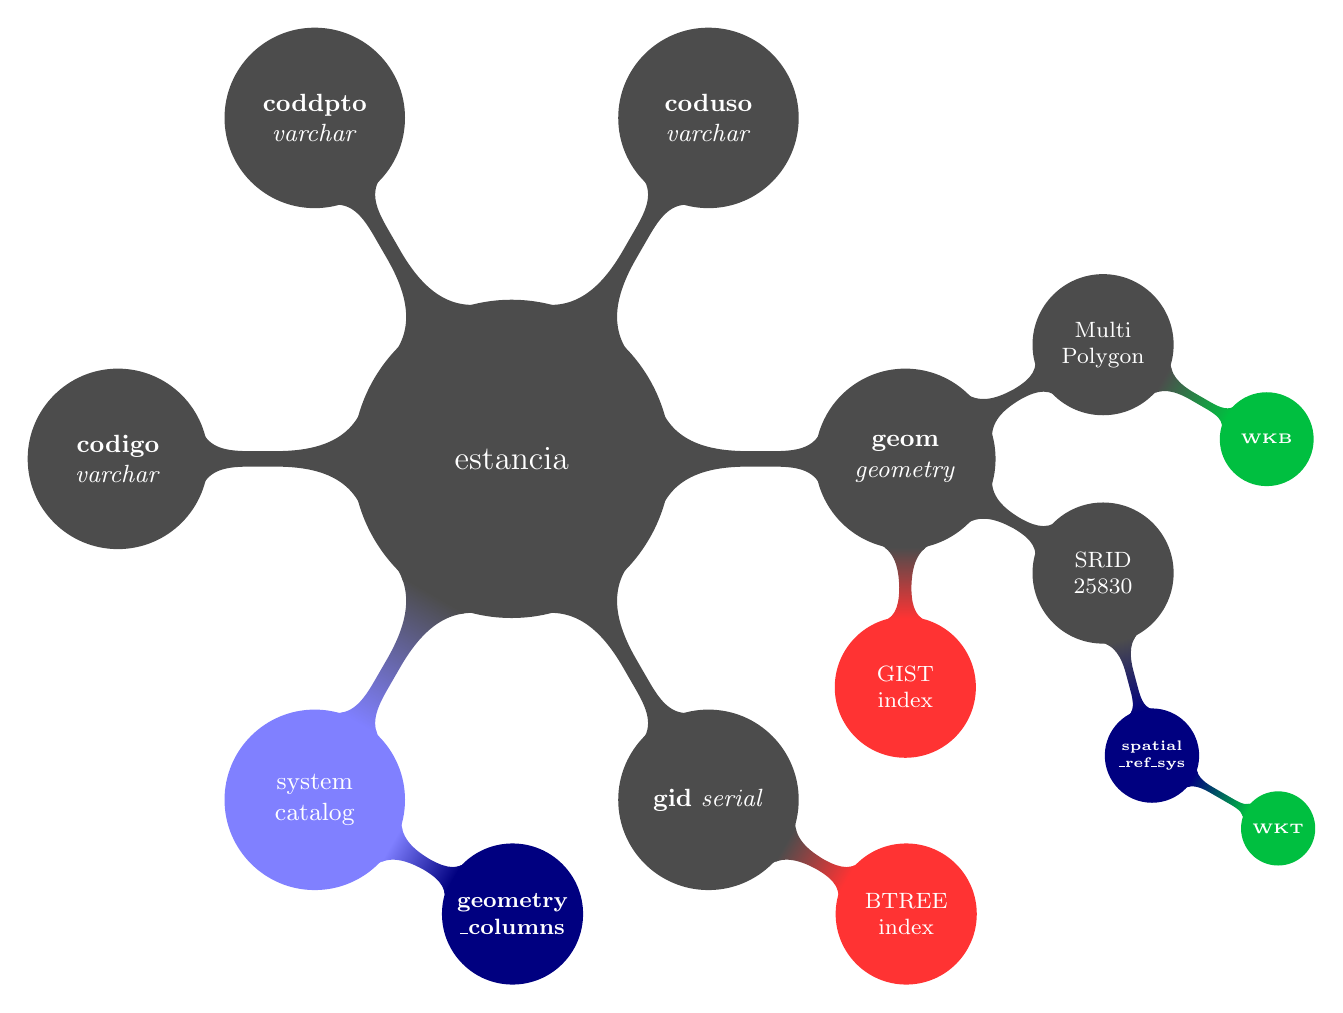
\begin{tikzpicture}
  \path[mindmap,concept color=black!70!white,text=white]
    node[concept] {estancia}
    [clockwise from=0]
    child {
      node[concept] {\textbf{geom} \textit{geometry}}
      [clockwise from=30]
      child { 
        node[concept] {Multi Polygon} 
        [clockwise from=-30]
        child[concept color=green!75!blue] { node[concept] {\textbf{WKB}} }
      }
      child { 
        node[concept] {SRID 25830} 
        [clockwise from=-75]
        child[concept color=blue!50!black] { 
          node[concept] {\textbf{\textbf{spatial \_ref\_sys}}} 
          [clockwise from=-30]
          child[concept color=green!75!blue] { node[concept] {\textbf{WKT}} }
        }
      }
      child[concept color=red!80!white] { node[concept] {GIST index} }
    }  
    child {
      node[concept] {\textbf{gid} \textit{serial}}
      [clockwise from=-30]
      child[concept color=red!80!white] { node[concept] {BTREE index} }
    }
    child [concept color=blue!50!white] {
      node[concept] {system catalog}
      [clockwise from=-30]
      child[concept color=blue!50!black] { node[concept] {\textbf{geometry \_columns}} }    
    }
    child { node[concept] {\textbf{codigo} \textit{varchar}} }
    child { node[concept] {\textbf{coddpto} \textit{varchar}} }
    child { node[concept] {\textbf{coduso} \textit{varchar}} };
\end{tikzpicture}}
\end{center}
\end{frame}

%%%%%%%%%%%%%%%%%%%%%%%%%%%%%%%%%%%
\section[Geometría]{El tipo geometry}
\subsection{PostGIS: la geometría de los datos geográficos}

\begin{frame}{El tipo de datos ``geometry''}
\begin{block}{Representación de geometrías según ISO 19125-2}
\begin{tikzpicture}
\umlsimpleclass[type=abstract]{Geometry} 
\umlsimpleclass[y=-2]{Point} 
\umlsimpleclass[x=2.5,y=-2]{LineString} 
\umlsimpleclass[x=5,y=-2]{Polygon} 
\umlinherit{Point}{Geometry}
\umlinherit{LineString}{Geometry}
\umlinherit{Polygon}{Geometry}

\end{tikzpicture}
\end{block}
\end{frame}

\end{document}
